\documentclass[notitlepage, reprint, nofootinbib]{revtex4-1}
\usepackage[utf8]{inputenc}

% Mathematics and symbols:
\usepackage{amsmath, gensymb, amsthm, physics, mhchem}
% Figures:
\usepackage{tikz, graphicx}
\usepackage[caption=false]{subfig}

% Other:
\usepackage{hyperref}


% Document formatting 
\setlength{\parskip}{1mm}
\setlength{\parindent}{0mm}

% Programming
\definecolor{codebackground}{rgb}{0.9,0.9,0.9}
\usepackage{listings}
\lstset{
	language=python,
	backgroundcolor=\color{codebackground},
	basicstyle=\scriptsize,
	aboveskip={1\baselineskip},
	columns=fixed,
	numbers=left,
	showstringspaces=false, 
	breaklines=true, 
	frame=single,
	showtabs=false,
	showspaces=false,
	keywordstyle=\color[rgb]{0,0,1},
	commentstyle=\color[rgb]{0.133,0.545,0.133}
	}

%\renewcommand{\thesubsubsection}{\alph{subsubsection})}

\hypersetup{
    colorlinks=true,
    linkcolor=blue,
    filecolor=magenta,      
    urlcolor=cyan,
}

\begin{document}
\title{FYS3150 - Project 1}
\author{Frida Larsen}

% Abstract
\begin{abstract}
This report investigates the difference between the Thomas algorithm, a more specialized version of the Thomas algorithm and the method of LU-decomposition for solving a linear matrix equation involving a tridiagonal matrix. Although the specialized version is the fastest, both it and the general Thomas algorithm are only applicable to tridiagonal matrices. For very small matrices, all three algorithms were subject to large timing errors due to the granularity of the CPU clock. The LU-decomposition method was the slowest and became useless for large grid sizes due to memory consumption and a high number of floating point operations. 
\end{abstract}

\maketitle

% Introduction
\section{Introduction}
There are many ways to approach a given problem, and many possible ways for reaching a solution. The aim of this project is to investigate and compare three different methods of solving the same problem, primarily in terms of numerical accuracy.\\[2mm]
Three algorithms will be employed to solve a matrix equation, the Thomas algorithm, a specialized version of the Thomas algorithm and the method of LU-decomposition. The equation in question is the one-dimensional Poisson equation, which is given by 
\begin{equation}\label{Poisson}-\dv[2]{x} u(x)=f(x),\end{equation}
with Dirichlet boundary conditions
\begin{equation}\label{Dirichlet}u(0)=u(1)=0\end{equation}
on the interval $x\in (0,1)$. \\[2mm]
We will start by discretizing and rewriting this equation as a matrix equation, before moving on to develop the algorithms for solving it.\\[2mm]
All relevant code may be found in the GitHub repository 'FYS3150-Computational-Physics'\footnote{\href{GitHub Repository}{https://github.com/fridalarsen/FYS3150-Computational-Physics}} under the Project1 folder. This folder also includes a Figures folder, which holds all the figures presented in this text as well as some additional figures.

% Theory
\section{Theory}
The second derivative of a general discretized function $g_i$ can be approximated by 
\begin{equation}\label{second_derivative} g_i'' \approx \frac{g_{i+1}+g_{i-1}-2g_i}{h^2}\end{equation}
The discretized version of the Poisson equation (\ref{Poisson}) then becomes 
\begin{equation}\label{Poisson_discrete}-\frac{u_{i+1}+u_{i-1}-2u_i}{h^2}=f_i,\end{equation}
where we have defined the discretized approximation to $u$ and $x$ as $u_i$ and $x_i$ respectively, such that $x_i=ih$, $x_0=0$ and $x_{n+1}=1$. We also have $f_i=f(x_i)$. The step length $h$ is defined as 
\begin{equation}\label{step_length}h=\frac{1}{n+1},\end{equation}
where $n$ is the total number of grid points on the interval (0,1). The discretized Dirichlet boundary conditions (\ref{Dirichlet}) are
\begin{equation}\label{Dirichlet2}u_0=u_{n+1}=0.\end{equation}
The discrete Poisson equation can be further simplified to
$$-u_{i+1}-u{i-1}+2u_i=h^2f_i.$$
By introducing $\tilde{d}_i=h^2f_i$ and remembering that $u_0=0$ the Poisson equation for the first few $i$-values are
\begin{align*}
	i=1:&\quad 2u_1-u_2=\tilde{d}_1\\
	i=2:&\quad -u_1+2u_2-u_3=\tilde{d}_2\\
	i=3:&\quad -u_2+2u_3-u_4=\tilde{d}_3\\
	&\dots
\end{align*}
This set of equations can be rewritten as a matrix equation 
\begin{equation}\label{lil_boi}\vb{A}\vb{u}=\vb{\tilde{d}}\end{equation}
with
\begin{equation}\label{big_boi}\vb{A}=\mqty( 2 & -1  & 0 &\dots &\dots &0\\-1&2&-1&0&\dots&\dots\\0&-1&2&-1&0&\dots\\ \dots&\dots&\dots&\dots&\dots&\dots \\ 0&\dots&\dots&-1&2&-1\\ 0&\dots&\dots&0&-1&2 ).\end{equation}
\newpage
\subsection{LU-decomposition}
Any square matrix may be factorized by LU-decomposition such that 
\begin{equation}\label{LU}\vb{P}\vb{M}_{(n\times n)}=\vb{L}\vb{U},\end{equation}
where $\vb{L}$ and $\vb{U}$ are lower and upper triangular matrices respectively. The matrix $\vb{P}$ is a permutation matrix, which describes the row permutations required on $\vb{M}$ for the LU-decomposition to be backwards compatible. \\[2mm]
In order to solve a linear matrix equation (like equation \ref{lil_boi}) one can use the LU-decomposition of the matrix by rewriting the equation as
\begin{equation}\label{LU_lil_boi}\vb{L}\vb{U}\vb{u}=\vb{P}\vb{\tilde{d}},\end{equation}
given $\vb{P}\vb{A}=\vb{L}\vb{U}$. There are then two steps to solving the equation; First solve $\vb{L}\vb{y} = \vb{P}\vb{\tilde{d}}$ for $\vb{y}$ and then finally $\vb{U}\vb{x} =\vb{y}$ for $\vb{x}$. 

% Method
\section{Method}
\subsection{The Thomas Algorithm}
The first algorithm we will be employing is known as the Thomas algorithm\cite{algo1} or the tridiagonal matrix algorithm. The algorithm is a two-step process involving a forward substitution and a backward substitution, and aims to solve equation \ref{lil_boi} where $\vb{A}$ is the general tridiagonal $n\times n$ matrix 
\begin{equation}\label{big_boi_bro}\vb{\tilde{A}} = \mqty(b_1&c_1&0&\dots&\dots&\dots\\a_1&b_2&c_2&0&\dots&\dots\\0&a_2&b_3&c_3&0&\dots\\ \dots&\dots&\dots&\dots&\dots&\dots\\ \dots&\dots&0&a_{n-2}&b_{n-1}&c_{n-1}\\ \dots&\dots&\dots&0&a_{n-1}&b_n)\end{equation}
The first step is given by  
\begin{equation}c_i' =\begin{cases} \frac{c_i}{b_i}&; \quad i=1\\ \frac{c_i}{b_i-a_ic_{i-1}'}&;\quad i=2,3,\dots,n-1\end{cases}\end{equation}
and 
\begin{equation}\tilde{d}_i'=\begin{cases}\frac{\tilde{d}_i}{b_i}&;\quad i=1\\ \frac{\tilde{d}_i-a_i\tilde{d}_{i-1}'}{b_i-a_ic_{i-1}'}&;\quad i=2, 3,\dots,n\end{cases}\end{equation}
This requires 2 floating point operations (FLOPs) for \ \ $i=1$, $3(n-1)$ FLOPs for the remaining $c_i'$'s and $5n$ FLOPs for the remaining $\tilde{d}_i'$'s.\\[2mm]
The second step is given by
\begin{align}
	u_n=\tilde{d}_n'&; \quad i=n\\
	u_i=\tilde{d}_i'-c_i'u_{i+1}&;\quad i=n-1,n-2,\dots,1.
\end{align}
This substitution requires 1 FLOP for $i=n$ and $2(n-1)$ FLOPs for the remaining computations. The total number of floating point operations for the Thomas algorithm is then
\begin{equation}\label{FLOP_thomas} \text{FLOPs} = (10n-2) \propto \order{n}.\end{equation}
\subsection{The Specialized Thomas Algorithm }
Although the Thomas algorithm is specialized for tridiagonal matrices, it does not take into account the equal elements along the diagonals of $\vb{A}$ (\ref{big_boi}), nor the fact that the upper and lower diagonals are equivalent. A more accurate generalization of the original matrix would be 
\begin{equation}\label{another_big_boi}\vb{A}_g = \mqty(b_1&a_1&0&0&\dots&0\\a_2&b_2&a_2&0&\dots&0\\0&a_3&b_3&a_3&\dots&0\\ 0&\dots&\dots&\dots&\dots&\dots\\ \dots&\dots&\dots&\dots&\dots&a_{n-1}\\ \dots&\dots&\dots&\dots&a_n&b_n),\end{equation}
where all $a_i=a$ and $b_i=b$. We observe that 
$$\vb{A}_g\ \ \mqty{\uppercase\expandafter{\romannumeral 2}-\frac{a_2}{b_2}\uppercase\expandafter{\romannumeral 1}\\ \sim}\ \mqty(b_1&a_1&0&0&\dots&0\\0&\tilde{b}_2&a_2&0&\dots&0\\0&a_3&b_3&a_3&\dots&0\\ 0&\dots&\dots&\dots&\dots&\dots\\ \dots&\dots&\dots&\dots&\dots&a_{n-1}\\ \dots&\dots&\dots&\dots&a_n&b_n),$$
with $\tilde{b}_2=b_2-\frac{a_2a_1}{b_1}$. Repeating this process for all rows 1 through $n$ removes the lower diagonal and replaces the diagonal elements by
\begin{equation}\label{b_tilde_ein} \tilde{b}_i=\begin{cases} b_1, \quad &i=1 \\ b_i - \frac{a_i a_{i-1}}{\tilde{b}_{i-1}},\quad &i=2, 3,\dots, n\end{cases}\end{equation}
Applying this process to the right hand side of equation \ref{lil_boi} results in
\begin{equation}\label{d_tilde_ein}\tilde{d}_i'=\begin{cases}\tilde{d}_1,\quad &i=1\\ \tilde{d}_i-\frac{a_i \tilde{d}_{i-1}'}{\tilde{d}_{i-1}'},\quad&i=2,3,\dots,n\end{cases}\end{equation}
Backward-substituting these expressions into equation {\ref{lil_boi}} yields
\begin{equation}\label{general_u_ein}u_i=\begin{cases}\frac{\tilde{d}_i'}{\tilde{b}_i},\quad&i=n\\ \frac{\tilde{d}_i'-a_i u_{i+1}}{\tilde{b}_i},\quad&i=n-1,n-2,\dots,1\end{cases}\end{equation}
Using the fact that our original matrix (\ref{big_boi}) has $a=-1$ and $b=2$, we get
\begin{align}
	\tilde{b}_i &= \begin{cases}2,\quad&i=1\\2-\frac{1}{\tilde{b}_{i-1}},\quad&i=1,2,\dots,n\end{cases}\nonumber\\
	&=\frac{i+1}{i},\quad \quad \quad \ \ \ i=1,2,\dots, n,\label{algo2b}
\end{align}
which leads to
\begin{align}
	\tilde{d}_i'&=\begin{cases}\tilde{d}_1,\quad &i=1\\\tilde{d}_i+\frac{\tilde{d}_{i-1}'}{i/(i-1)},\quad&i=2,3,\dots, n\end{cases}\nonumber\\
	&=\tilde{d}_i+\frac{(i-1)\tilde{d}_{i-1}'}{i},\quad i=1,2,\dots,n.\label{algo2f}
\end{align}
This forward substitution requires $2n$ and $4n$ FLOPs for calculating the $\tilde{b}_i$'s and $\tilde{d}_i'$'s respectively. The final solution is then ultimately found by backwards substitution,
\begin{equation}\label{algo2u}u_{i-1}=\frac{i-1}{i}(\tilde{d}_{i-1}'+u_i),\ i=n-1,\dots,2\end{equation}
with $u_n=\tilde{d}_n'/\tilde{b}_n$. This requires $1 + 4(n-1)$ FLOPs, which means that the specialized algorithm has a total number of FLOPs given by 
\begin{equation}\label{FLOPS_special} \text{FLOPs}=9n-3\propto \order{n}.\end{equation}
\subsection{LU-decomposition}
In order to solve equation \ref{lil_boi} using LU-decomposition we will implement the functions \texttt{lu\_factor} and \texttt{lu\_solve} from SciPy's Linalg Library\cite{SciPy_linalg}. 
\subsection{Comparison}
In order to test these algorithms, we will use a function for the right hand side of equation \ref{Poisson} given by
\begin{equation}\label{test_func}f(x)= 100e^{-10x},\end{equation}
which has closed-form solution 
\begin{equation}\label{test_func_sol}u_s(x)=1-(1-e^{-10})x-e^{-10x}.\end{equation}
In addition to comparing the algorithms' solutions, we will also compare their CPU times for several grid sizes $n$. 
% Results
\section{Results}
Figures \ref{1a} and \ref{1b} compare the solution of the Thomas algorithm to the analytic solution for matrix sizes $n=10$ and $n=100$. Figure \ref{1c} compares the solution of the specialized algorithm to the analytic solution for a matrix of size $n=100$. The relative errors of the specialized algorithm for different values of $n$ are presented in table \ref{error_table}. \\[2mm]
\newpage
\begin{table}[h!]
\centering
\begin{tabular}{|c|c|c|c|c|c|c|}
\hline
Grid size, $n$ & 1e1 & 1e2 & 1e3 & 1e4 & 1e5 & 1e6 \\ \hline
Relative error & -1.18 & -3.09 & -5.08 & -7.08 & -9.08 & -10.16 \\ \hline
\end{tabular}
\caption{Logarithmic relative error of the specialized Thomas algorithm for different matrix sizes, $n$.}
\label{error_table}
\end{table}
Figure \ref{1d} compares the solution of the LU-decomposition method to the analytic solution for a matrix of size $n=100$. We note that while the Thomas algorithms support $n>10^5$, it was impossible to run the LU-decomposition method for matrices of size $n=10^5$ or larger.\\[2mm]
Figure \ref{fig3} shows the average CPU run times for the three methods with the standard deviations indicated as error-bars. The average was taken over 5 runs. Note that the horizontal lines are not error-bars, but a consequence of the errors being very small. We observe that the Thomas algorithm and the special Thomas algorithm both have a linear relationship between $n$ and the run time, whilst the LU-decomposition method does not. The latter has a more rapid growth than a linear relationship would. We also observe that the lower $n$-values have a larger uncertainty in time.

% Discussion
\section{Discussion}
All the algorithms used in this project managed to reproduce the closed-form solution for matrix sizes $n\geq 100$. This is reflected in the relative errors for the specialized Thomas algorithm, table \ref{error_table}, where we saw that the error became significantly smaller as the grid size increased. \\[2mm]
From the CPU times (figure \ref{fig3}) we saw that the LU-decomposition method was significantly slower than the other two methods, particularly for the larger grid sizes. In particular, the LU-decomposition method was unable to run on a standard laptop for matrix sizes above $n=10^5$, without using hard drive memory. There are two aspects of the LU-decomposition method that may explain this.\\[2mm]
First, the number of floating point operations required by the LU-decomposition method is of order $n^3$\cite{lecture_notes}. This is a very large number compared to the other two algorithms, both of which only require $\order{n}$ floating point operations. This results in the LU-decomposition method being much slower for large $n$.\\[2mm]
Second, the SciPy functions that performs the LU-decomposition and solves the matrix equation continually fetch and store matrix elements. This causes the functions to use significantly more memory than the Thomas algorithms, which in turn results in the method being unusable for large values of $n$. There simply isn't enough RAM on an ordinary laptop for handling $n\geq10^5$. 
\onecolumngrid 
\clearpage
\begin{center}\begin{figure}[]
	\centering
	\subfloat[Thomas algorithm, $n=10$.]{\label{1a}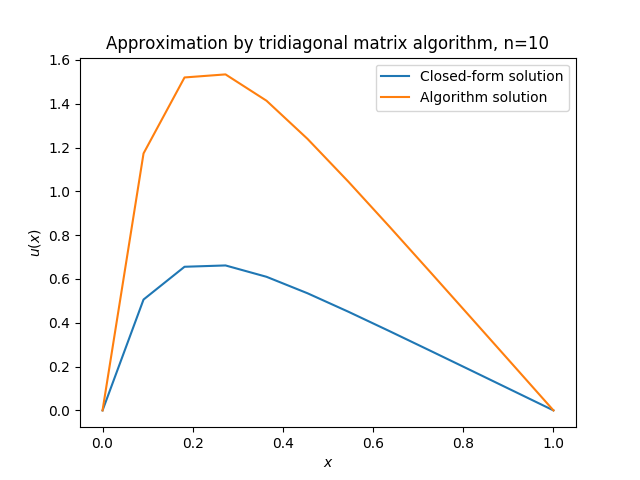
\includegraphics[width=0.5\textwidth]{../Figures/t_m_a_n_10.png}}
	\subfloat[Thomas algorithm, $n=100$.]{\label{1b}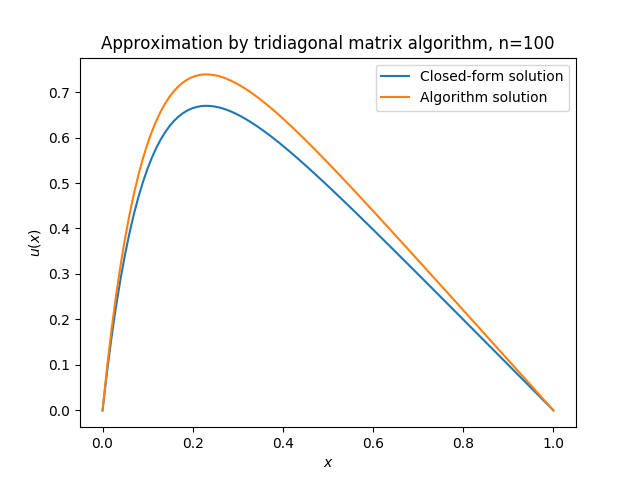
\includegraphics[width=0.5\textwidth]{../Figures/t_m_a_n_100.png}}
	\\
	\subfloat[Specialized Thomas algorithm, $n=100$.]{\label{1c}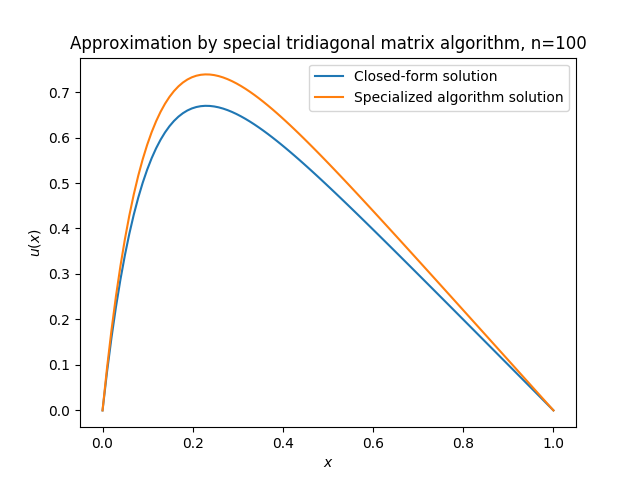
\includegraphics[width=0.5\textwidth]{../Figures/stma_n100.png}}
	\subfloat[LU-decomposition method, $n=100$.]{\label{1d}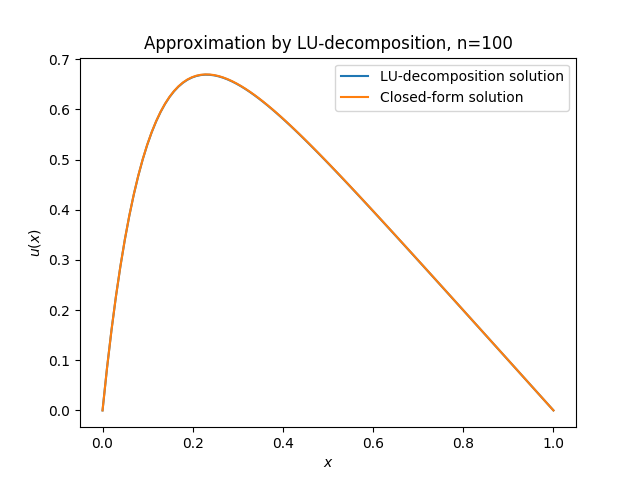
\includegraphics[width=0.5\textwidth]{../Figures/LU_decomp_100.png}}
	\caption{Comparison of the algorithm solution and the analytical solution for the function $f$ (\ref{test_func}) for different sized matrices.}
	\label{fig1}
\end{figure}\end{center}
\clearpage
\twocolumngrid
The strength of the Thomas algorithms is their use of the tridiagonal matrix symmetries. This makes them able to solve the problem for larger grid sizes, where the LU-decomposition method fails. On the other hand, this makes them suitable for specific cases only, while the LU-decomposition method can be used in a larger variety of cases.\\[2mm]
An aspect of all three methods with regards to the CPU times was a significantly larger error in the times for small $n$-values. The calculations for small grid sizes were a lot faster than those for larger grids. In fact, the runtimes were comparable to the CPU clock's granularity. The clock's precision simply wasn't high enough to capture the rapid calculation time. \\[2mm]
The relationship between runtimes and number of floating point operations appears to be proportional. As mentioned above, whereas the Thomas algorithms perform $\order{n}$ floating point operations, the LU-decomposition method requires $\order{n^3}$. This is reflected in the runtime plots. The Thomas algorithms both have a linear relationship between the time required and $n$, while the LU-decomposition method grows faster. 
% Conclusion
\section{Conclusion}
The aim of this project was to explore the precision and differences of the three algorithms presented. Overall, we found that the fastest algorithm was the special algorithm because it took into account the symmetries and particularities of the problem. The more general algorithms might be able to solve a larger variety of problems, but they are significantly slower in doing so. \\[2mm]
We also found that solving problems numerically requires awareness of the inherent limitations of ordinary laptops. Aspects such as available memory and decimal precision may cause unpredicted problems.
\onecolumngrid
\begin{center}\begin{figure}[t]
	\centering
	\subfloat[Generalized and specialized Thomas algorithms.]{\label{3a}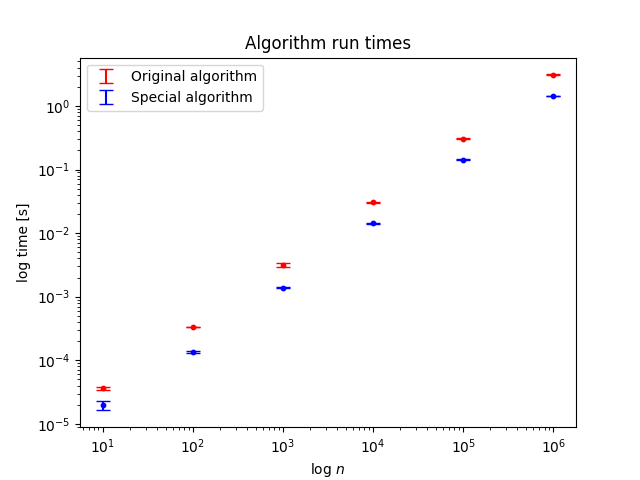
\includegraphics[width=0.45\textwidth]{../Figures/time_plot.png}}
	\subfloat[LU-decomposition algorithm.]{\label{3b}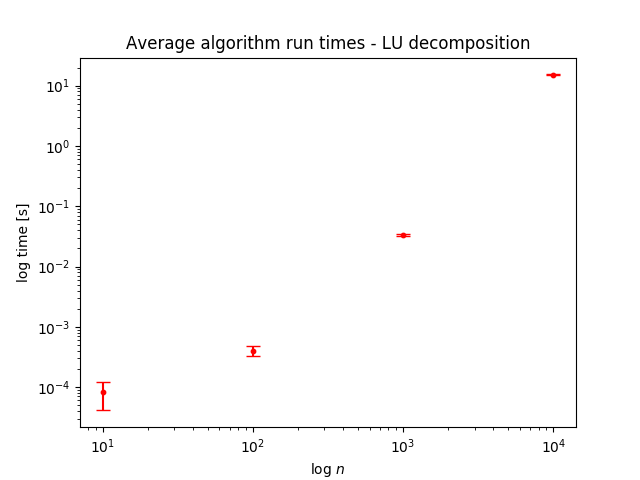
\includegraphics[width=0.45\textwidth]{../Figures/time_plot_LU.png}}
	\caption{Log-log plots of the average time consumed by the three algorithms as a function of grid size $n$ with errors.}
	\label{fig3}
\end{figure}\end{center}
\twocolumngrid
% Bibliography
\onecolumngrid
\bibliographystyle{unsrtnat}
\bibliography{references.bib}

















\end{document}